\documentclass[tikz,border=12pt]{standalone}
\usepackage[T1]{fontenc}
\usepackage{mathpazo}
\usepackage{amsmath,amssymb}
\usetikzlibrary{arrows.meta, positioning, calc, fit, decorations.pathreplacing}

\definecolor{stblue}{HTML}{7B97AD}
\definecolor{rwgold}{HTML}{B8995E}
\definecolor{sage}{HTML}{7A9A7E}
\definecolor{dkbrown}{HTML}{3D3530}
\definecolor{wmgray}{HTML}{7B7067}
\definecolor{cream}{HTML}{F9F6F0}
\definecolor{border}{HTML}{D4C9B8}
\definecolor{terracotta}{HTML}{C47A6A}
\definecolor{lavender}{HTML}{907EA0}

\begin{document}
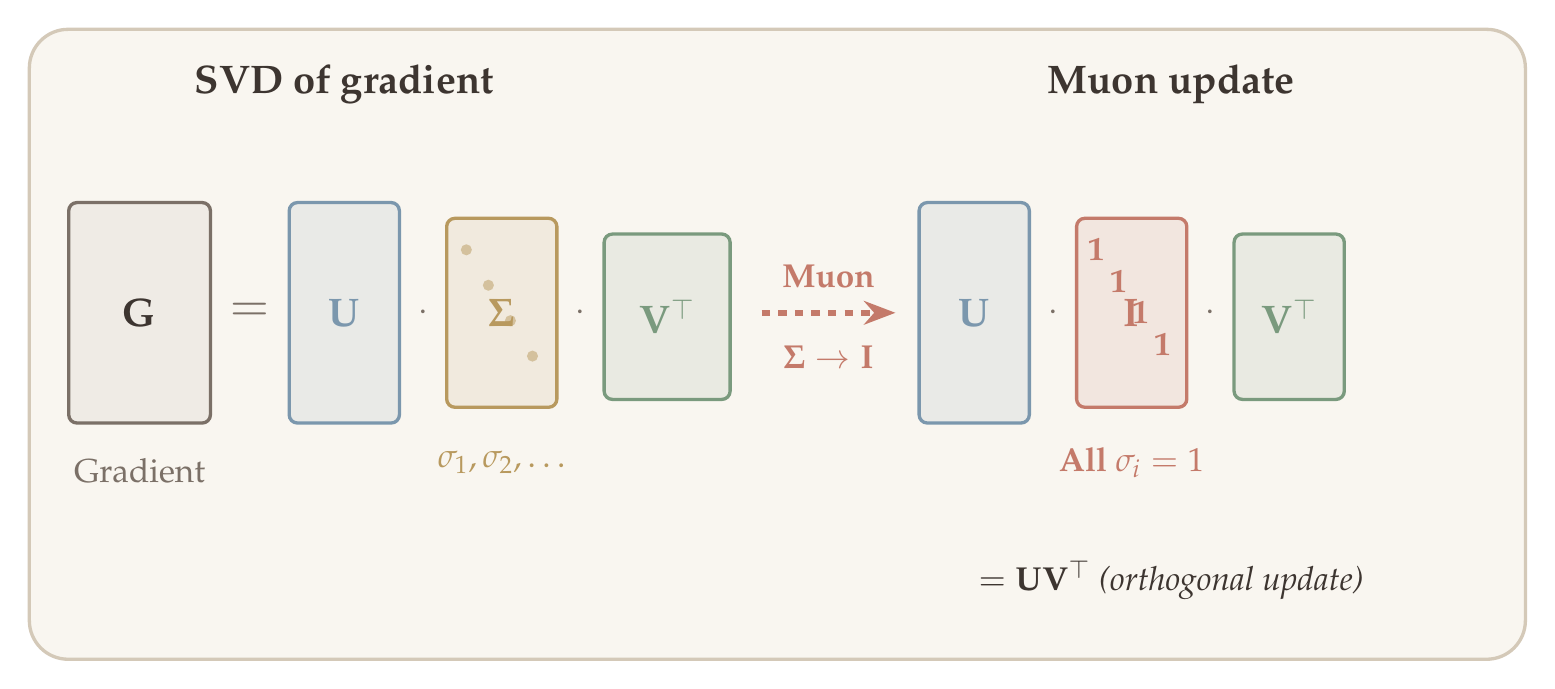
\begin{tikzpicture}[>={Stealth[length=4mm, width=3mm]}, line width=1.5pt]

% Background
\fill[cream, rounded corners=14pt] (-0.5,-2.0) rectangle (18.5,6.0);
\draw[border, line width=1.2pt, rounded corners=14pt] (-0.5,-2.0) rectangle (18.5,6.0);

% Top labels
\node[text=dkbrown, font=\Large\bfseries] at (3.5,5.3) {SVD of gradient};
\node[text=dkbrown, font=\Large\bfseries] at (14.0,5.3) {Muon update};

% G matrix
\draw[wmgray, line width=1.2pt, rounded corners=3pt] (0.0,1.0) rectangle (1.8,3.8);
\fill[wmgray, opacity=0.08, rounded corners=3pt] (0.0,1.0) rectangle (1.8,3.8);
\node[text=dkbrown, font=\Large\bfseries] at (0.9,2.4) {$\mathbf{G}$};
\node[text=wmgray, font=\large] at (0.9,0.4) {Gradient};

% = sign
\node[text=wmgray, font=\LARGE] at (2.3,2.4) {$=$};

% U matrix (blue)
\draw[stblue, line width=1.2pt, rounded corners=3pt] (2.8,1.0) rectangle (4.2,3.8);
\fill[stblue, opacity=0.12, rounded corners=3pt] (2.8,1.0) rectangle (4.2,3.8);
\node[text=stblue, font=\Large\bfseries] at (3.5,2.4) {$\mathbf{U}$};

% dot
\node[text=wmgray, font=\large] at (4.5,2.4) {$\cdot$};

% Sigma matrix (gold)
\draw[rwgold, line width=1.2pt, rounded corners=3pt] (4.8,1.2) rectangle (6.2,3.6);
\fill[rwgold, opacity=0.12, rounded corners=3pt] (4.8,1.2) rectangle (6.2,3.6);
\node[text=rwgold, font=\Large\bfseries] at (5.5,2.4) {$\boldsymbol{\Sigma}$};
% diagonal dots
\foreach \i/\y in {0/3.2, 1/2.75, 2/2.3, 3/1.85} {
  \fill[rwgold, opacity=0.5] (5.05+\i*0.28, \y) circle (2pt);
}
\node[text=rwgold, font=\large] at (5.5,0.5) {$\sigma_1, \sigma_2, \ldots$};

% dot
\node[text=wmgray, font=\large] at (6.5,2.4) {$\cdot$};

% V^T matrix (green)
\draw[sage, line width=1.2pt, rounded corners=3pt] (6.8,1.3) rectangle (8.4,3.4);
\fill[sage, opacity=0.12, rounded corners=3pt] (6.8,1.3) rectangle (8.4,3.4);
\node[text=sage, font=\Large\bfseries] at (7.6,2.35) {$\mathbf{V}^\top$};

% Long arrow: Muon replaces Sigma with I
\draw[terracotta, ->, line width=2pt, dashed] (8.8,2.4) -- (10.5,2.4);
\node[text=terracotta, font=\large\bfseries, above=2pt] at (9.65,2.5) {Muon};
\node[text=terracotta, font=\large, below=2pt] at (9.65,2.2) {$\boldsymbol{\Sigma} \to \mathbf{I}$};

% U matrix copy (blue)
\draw[stblue, line width=1.2pt, rounded corners=3pt] (10.8,1.0) rectangle (12.2,3.8);
\fill[stblue, opacity=0.12, rounded corners=3pt] (10.8,1.0) rectangle (12.2,3.8);
\node[text=stblue, font=\Large\bfseries] at (11.5,2.4) {$\mathbf{U}$};

% dot
\node[text=wmgray, font=\large] at (12.5,2.4) {$\cdot$};

% I matrix (rose)
\draw[terracotta, line width=1.2pt, rounded corners=3pt] (12.8,1.2) rectangle (14.2,3.6);
\fill[terracotta, opacity=0.12, rounded corners=3pt] (12.8,1.2) rectangle (14.2,3.6);
\node[text=terracotta, font=\Large\bfseries] at (13.5,2.4) {$\mathbf{I}$};
% diagonal ones
\foreach \i/\y in {0/3.2, 1/2.8, 2/2.4, 3/2.0} {
  \node[text=terracotta, font=\large\bfseries] at (13.05+\i*0.28, \y) {1};
}
\node[text=terracotta, font=\large\bfseries] at (13.5,0.5) {All $\sigma_i = 1$};

% dot
\node[text=wmgray, font=\large] at (14.5,2.4) {$\cdot$};

% V^T matrix copy (green)
\draw[sage, line width=1.2pt, rounded corners=3pt] (14.8,1.3) rectangle (16.2,3.4);
\fill[sage, opacity=0.12, rounded corners=3pt] (14.8,1.3) rectangle (16.2,3.4);
\node[text=sage, font=\Large\bfseries] at (15.5,2.35) {$\mathbf{V}^\top$};

% Result label
\node[text=dkbrown, font=\large\itshape] at (14.0,-1.0) {$= \mathbf{U}\mathbf{V}^\top$ (orthogonal update)};

\end{tikzpicture}
\end{document}
